\documentclass[submit]{harvardml}

% Put in your full name and email address.
\name{Luke Mueller}
\email{lam908@mail.harvard.edu}

% List any people you worked with.
\collaborators{%
	Nicole Lee,
	Dong Yan
}

% You don't need to change these.
\course{CS181-S16}
\assignment{Assignment \#2}
\duedate{5:00pm February 26, 2016}

\usepackage[OT1]{fontenc}
\usepackage[colorlinks,citecolor=blue,urlcolor=blue]{hyperref}
\usepackage[pdftex]{graphicx}
\usepackage{subfig}
\usepackage{fullpage}
\usepackage{palatino}
\usepackage{mathpazo}
\usepackage{amsmath}
\usepackage{amssymb}
\usepackage{color}
\usepackage{todonotes}
\usepackage{listings}
\usepackage{common}
\usepackage{bm}

\usepackage[mmddyyyy,hhmmss]{datetime}

\definecolor{verbgray}{gray}{0.9}

\lstnewenvironment{csv}{%
  \lstset{backgroundcolor=\color{verbgray},
  frame=single,
  framerule=0pt,
  basicstyle=\ttfamily,
  columns=fullflexible}}{}

\begin{document}
\begin{center}
{\Large Homework 2: Linear Classification}\\
\end{center}

There is a mathematical component and a programming
component to this homework. Please submit your PDF to Canvas, and push everything in Github.

This homework is about multi-class classification. Whereas in more simple
classification models we build classifiers that discriminate between two classes,
in multi-class regression, we discriminate between three or more classes.  As
usual, we imagine that we have the input matrix $\boldX \in \reals^{N \times D}$
(or perhaps they have been mapped to some basis $\bm{\Phi}$, without loss
of generality) but that our outputs are now ``one-hot coded''.  What that means
is that, if there are~$K$ output classes, rather than representing the output
labels as integers~${1,2,\ldots,K}$, we represent them as a binary vectors of
length~$K$.  These vectors are zero in each component except for the one
corresponding to the correct label, and that entry has a one.  So, if there are
7 classes and a particular datum has label 3, then the target vector would
be~${[0,0,1,0,0,0,0]}$ (assuming the labels are 1-indexed).

In the first problem, you will be exploring the properties of the softmax
function, which is central to multiclass logistic regression.  In the second
problem, we will have you dive into the matrix algebra and methods behind
generative classifications.  Finally, in the third problem, you will implement a
generative classifier and logistic regression from close to scratch, and the
first two problems should inform this!

%\subsection*{1. Properties of Softmax [5pts]}
%%%%%%%%%%%%%%%%%%%%%%%%%%%%%%%%%%%%%%%%%%%%%
% Problem 1
%%%%%%%%%%%%%%%%%%%%%%%%%%%%%%%%%%%%%%%%%%%%%
\begin{problem}[Properties of Softmax , 5pts]

Logistic regression is a discriminative probabilistic model: a prediction
consists of a distribution over the different classes. In other words, logistic
regression outputs a vector of nonnegative numbers that sum to one.

The softmax function generalizes the logistic sigmoid to the case of $K$
classes: it takes as input a vector, and outputs a K dimensional vector in the
range $[0,1]$ whose components sum to $1$:

\[ \bm{\sigma}(\mathbf{z}) = softmax(\mathbf{z}) =
\frac{\exp(\mathbf{z})}{\sum_i\exp(z_i)}\]

In logistic regression, we often use the softmax-based parameterization over $K$ vectors $\{\boldw_k\}$:

\begin{align*}
  \Pr(t_{nk}=1 \given \boldX, \{\boldw_{k'}\}^K_{k'=1})
  &= \frac{ \exp\{ \boldw_k^{\trans}\boldx_n \} }
  { \sum_{k'=1}^K \exp\{ \boldw_{k'}^{\trans}\boldx_n \} }\,.
\end{align*}

Here we're using~${t_{nk}=1}$ to indicate the probability that the $n$th entry
is assigned to the $k$th class.\\

Softmax is a crucial function in logistic regression, and you will see it again in other models, such as neural networks. 
So, we want you to start gaining the intuitions for the properties of softmax, and for common methods that employ it. 

Show that:
\begin{enumerate}
  \item The output of the softmax function is always a vector with non-negative components
    that are at most 1. 
  \item The output of the softmax function forms a distribution (the components sum to 1).
  \item Softmax preserves order. This means that if the elements of $\mathbf{z}$ have some order, then the elements of $\bm{\sigma}(\mathbf{z})$ have the same order. 
  \item Equation 4.106 from Bishop holds
  \item Using your answer to the previous question, show that equation 4.109
    holds. By the way, this may be useful for Problem 3!
\end{enumerate}
\end{problem}
\subsection*{Solution}

\begin{enumerate}
	\item The proof for this property of the softmax is fairly trivial. First, we choose the largest value of the vector $\mathbf{z}$, and call it $m=max(\mathbf{z})$. Then performing the $softmax$ function on $m$ we have:
		\[ \bm{\sigma}(m) = softmax(m) =
		\frac{\exp(m)}{\sum_i\exp(z_i)}\ =
		\frac{\exp(m)}{\sum_i\exp(m)+...+exp(z_n)}\]
	which will always be less than 1 since the exponential function is positive monotonic and $\frac{x}{x+y}<1$ where $y \neq x$. For completeness, the exponential function is positive monotonic since:
		\[\frac{\partial}{\partial x} exp(x) = exp(x)\]
	\item Taking sum of the outputs for each element of $\mathbf{z}$ gives us:
		 \[\frac{\exp(z_1)}{\sum_i\exp(z_i)}\ + ... +
		 \frac{\exp(z_k)}{\sum_i\exp(z_i)}\ =
		 \frac{\sum_i\exp(z_i)}{\sum_i\exp(z_i)}\ = 
		 1\]
	We also could have integrated over the softmax to prove this.
	\item Let  $\mathbf{z}$ have some order such that $\forall i<j$ where $i \neq j$, $z_i \leq z_j$. Thus we have $z_1<z_2<...<z_k$. Then if we use the softmax function elementwise on $\mathbf{z}$ we will have:
		 \[\frac{\exp(z_1)}{\sum_i\exp(z_i)}\ , ... ,
		 \frac{\exp(z_k)}{\sum_i\exp(z_i)}\]
	Since the denominator is the same for all softmax transformed elements we will only consider the numerator for comparing order. Again, since the exponential function is monotonic positive we have indeed preserved order. In particular, we have:
		\[z_i<z_j \Rightarrow exp(z_i) < exp(z_j)\]
	The converse of this property is similar proven:
		\[z_i>z_j \Rightarrow exp(z_i) > exp(z_j)\]
	\item Equation 4.106 in Bishop says that the derivative of the softmax with respect to its activations $a_j$ is:
		\[\frac{\partial y_k}{\partial a_j}\ =
		y_k (\mathbf{I}_{kj} - y_j) 
		\]
	where $y_k (\phi) = \frac{exp(a_k)}{\sum_j\exp(a_j)}$ and $a_k = {\mathbb{W}_k}^T\phi$ \\
	To prove this derivative, we consider two separate cases. First, where $j \neq k$ and second, where $j = k$. Thus for the first case we have:
		\[
		\frac{\partial y_k}{\partial a_j} \frac{exp(a_k)}{\sum_j exp(a_j)}, \
		k \neq j
		\]
	Since $k \neq j$ we can ignore the numerator and only differentiate the denominator, where only one element of the sum is of interest. Applying the chain rule we then have:
		\[
		\frac{\partial y_k}{\partial a_j} [\sum_j exp(a_j)]^{-1} = \
		\frac{-exp(a_j)exp(a_k)}{[\sum_j exp(a_j)]^2} = \
		y_k (-y_j) \
		\]
	Now for the second case, where $j=k$, we must consider both the numerator and denominator, necessitating use of the quotient rule. In particular, we set the numerator as $f(a_k)=exp(a_k)$ such that $f'(a_k)=exp(a_k)$, and the denominator as $g(a_j)=\sum_j exp(a_j)$ such that $g'(a_j)$ is the same expression derived above (without $exp(a_k)$ since it was a constant in that derivative). Then combining the two we have:
		\[
		[\frac{exp(a_k)}{\sum_j exp(a_j)} - \frac{exp(a_k)exp(a_j)}{[\sum_j exp(a_j)]^2}] \
		[\sum_j exp(a_j)]^2 \
		\]
	Then simplifying terms algebraically we have:
		\[
		exp(a_k)\sum_j exp(a_j) - \
		exp(a_k)exp(a_j) = \
		exp(a_k)[\sum_j exp(a_j)-exp(a_j)] \		
		\]
	Then dividing the equation by $\sum_j exp(a_j)$ we have:
		\[
		\frac{exp(a_k)}{\sum_j exp(a_j)} \
		[1-\frac{exp(a_j)}{\sum_j exp(a_j)} ] = \
		y_k (\mathbf{I}_{kj} - y_j) \
		\]
	where $\mathbf{I}_{kj}$ are elements of the identity matrix. The result thus explains both cases presented above.
	\item Equation 4.109 in Bishop says that the gradient of the error function with respect to one of the parameter vectors $\mathbf{W}_j$ is:
		\[
		\nabla_{\mathbf{W}_j} E(\mathbf{W}_1,...,\mathbf{W}_k) = \
		\sum_{n-1}^{N} (y_{nj}-t_{nj})\phi_n \
		\]
	The error function results from the negative log likelihood function and can be written as:
		\[
		E(\mathbf{W}_1,...,\mathbf{W}_k) = \
		-\sum_{n=1}^{N}\sum_{k=1}^{K} t_{nk}\ln y_{nk} \
		\]
	Again we consider two cases. First, where $j \neq k$ and second, where $j = k$. We will also use the result from (4), Bishop's equation 4.106 to explain the derivative of the softmax function. Thus for the first case we have:
		\[
		\nabla_{\mathbf{W}_j} E(\mathbf{W}_1,...,\mathbf{W}_k) = \
		\sum_{n=1}^{N}\frac{\frac{t_{nk}exp(a_j)\phi_n exp(a_k)}{[\sum_j exp(a_j)]^2}}{\frac{exp(a_k)}{\sum_j exp(a_j)}}  = \
		\sum_{n=1}^{N}\frac{t_{nk}exp(a_j)\phi_n}{\sum_j exp(a_j)} = \
		\sum_{n=1}^{N}y_{nj}\phi_n \
		\]
	where we have made use of $\sum_k t_{nk}=1$ \\
	Then for the second case, where $j=k$ we have:
		\[
		\nabla_{\mathbf{W}_j} = \
		-\sum_{n=1}^{N}t_{nj}\frac{\frac{exp(a_k)}{\sum_j exp(a_j)}
		[1-\frac{exp(a_j)\phi_n}{\sum_j exp(a_j)} ]}{\frac{exp(a_k)}{\sum_j exp(a_j)}} = \
		-\sum_{n=1}^{N} \frac{\sum_j exp(a_j)}{exp(a_k)} - \
		\frac{exp(a_j)\phi_n}{exp(a_k)} = \
		-\sum_{n=1}^{N}t_{nj}\frac{\sum_j exp(a_j) - exp(a_j)\phi_n} {exp(a_k)} \
		\]
	Then multiplying the inside of the sum by $y_{nk}$ we get:
		\[
		-\sum_{n=1}^{N}t_{nj}(1-\frac{exp(a_j)\phi_n}{\sum_j exp(a_j)}) = \
		-\sum_{n=1}^{N}t_{nj}(1-y_{nj}\phi_n)  = \
		\sum_{n-1}^{N} (y_{nj}-t_{nj})\phi_n \
		\]
	which, as in part (4), satisfies both cases.
\end{enumerate}


%\subsection*{2. Mooooar matrix calculus [10 pts]}
%%%%%%%%%%%%%%%%%%%%%%%%%%%%%%%%%%%%%%%%%%%%%
% Problem 2
%%%%%%%%%%%%%%%%%%%%%%%%%%%%%%%%%%%%%%%%%%%%%
\begin{problem}[Mooooar matrix calculus , 10pts]
\textbf{Note - this problem appears longer than it is, since we broke up one problem into separate parts rather
than having you do all of these steps at once. Many of these subparts may be just one or two lines.}\\

Consider a generative K-class model.  We define the class prior with vector
$\vec \pi$: $\mathbb{P}(\mathcal{C}_k) = \pi_k$.  We define the
class-conditional densities $\mathbb{P}(\phi|\mathcal{C}_k)$ where $\phi$ is the
input feature vector. Consider the data set $\{\phi_n, {\bf t}_n\}$ where $n = 1 \dots N$ where ${\bf
t}_n \in \{0,1\}^K$ is a one-hot encoded target vector. This means that
$\bf{t}_n$ is 0 everywhere, except for in the $k$th position, where $k$ is the
class assigned to the $n$th feature vector.
\begin{enumerate}
  \item Write out the complete-data log-likelihood of the data set using only the
    notations introduced in the problem formulation above.
    $$\ln \mathbb{P}(\{\phi_n, {\bf t}_n \} | \{\pi_k \}) =?$$
  \item Since the prior forms a distribution, it has the constraint that
    $\sum_k\pi_k - 1 = 0$.  Using the hint at the end of the exercise, give the
    expression for the maximum-likelihood estimator for the prior
    class-membership probabilities:
    $$\hat \pi_k =?$$
    Make sure to write out the intermediary equation you need
    to solve to obtain this estimator. Double-check your answer: the final
    result should be very intuitive!
\end{enumerate}
    We will suppose for the remaining questions of this exercise that the
    class-conditional probabilities are given by gaussian distributions with the
    same covariance matrix:
    $$\mathbb{P}(\phi | C_k) = \mathcal{N}(\phi | \vec \mu_k, \Sigma)$$
    \begin{enumerate}
  \item[3.] Write out the gradient of log-likelihood with respect to vector $\mu_k$.
    Write the expression in matrix form as a function of the variables defined
    throughout this exercise. Simplify as much as possible for full credit.
  \item[4.] Write out the maximum-likelihood estimator for vector $\mu_k$. Once
    again, your final answer should seem intuitive.
  \item[5.] Write out the gradient for the log-likelihood with respect to the
    covariance matrix $\Sigma$. Even though the log-likelihood function is a
    scalar function, since you are differentiating with respect to a
    \emph{matrix}, the resulting expression should be a matrix!
  \item[6.] Express the maximum likelihood estimator of the covariance matrix.
\end{enumerate}

\paragraph{Hint.} When maximizing a function $f$ with respect to an equality
constraint that needs to be met at the optimum (which can always be written as
$g(x) = 0$), we introduce a Lagrange multiplier $\lambda$ and maximize: $$\max_x
f(x) + \lambda g(x)$$

\paragraph{Cookbook formulas.} Here are some formulas you might want to consider
using to compute difficult gradients. You can use them as is in the homework
without proof. If you are looking to hone your matrix calculus skills, try to
find different ways to prove these formulas yourself (will not be part of the
evaluation of this homework). In general, you can use any formula from the matrix cookbook,
as long as you cite it. We opt for the following common notation:
$X^{-T} := (X^{-1})^{-T} = (X^{T})^{-1}$
\begin{align*}
  & \frac{\partial a^T X^{-1} b}{\partial X} = - X^{-T} a b^T X^{-T} \\
  & \frac{\partial \ln | \det (X) |}{\partial X} = X^{-T}
 \end{align*}
 \end{problem}

\subsection*{Solution}
\begin{enumerate}
	\item To write the complete-data log likelihood of the data set we will need the product of the priors and class-conditional densities for all classes $k$. Following Bishop's 2-class example in equation 4.89 we have:
	\[
	\ln \mathbb{P}(\{\phi_n, {\bf t}_n \} | \{\pi_k \}) = \
	\ln\prod_{n=1}^{N}\prod_{k=1}^{K}(\pi_k*\mathbb{P}(\phi|\mathbb{C}_k))^{t_{nk}} = \
	\sum_{n=1}^{N}\sum_{k=1}^{K}t_{nk}[\ln\mathbb{P}(\phi | C_k)]+\ln(\pi_k)] \
	\]
	\item To determine the maximum-likelihood estimator for the prior class-membership probabilities we take the derivative of the complete-data log likelihood shown above, with respect to $\pi_k$. Then to comply with the constraint  $\sum_k\pi_k - 1 = 0$ we will introduce a lagrange multiplier and maximize $\max_x f(x) + \lambda g(x)$ Thus we have:
	\[
	\frac{\partial}{\partial \pi_k} \
	\sum_{n=1}^{N}\sum_{k=1}^{K}t_{nk}\ln(\pi_k)+t_{nk}\ln(\mathbb{P}(\phi | C_k)) + \
	\lambda[\sum_k\pi_k - 1] \
	\]
	Then taking derivatives and simplifying we have:
	\[
	\sum_{n=1}^{N} \frac{t_{nk}}{\pi_k}+\lambda = \
	\frac{1}{\pi_k}\sum_{n=1}^{N} t_{nk} + \lambda \
	\]
	Then setting equal to $0$ and solving for $\pi_k$:
	\[
	\frac{1}{\pi_k}\sum_{n=1}^{N} t_{nk} + \lambda = 0 \Rightarrow \
	\hat \pi_k = -\frac{\sum_{n=1}^{N} t_{nk} }{\lambda} \
	\]
	Then taking the derivative with respect to $\lambda$:
	\[
	\frac{\partial}{\partial \lambda} \
	\ln \mathbb{P}(\{\phi_n, {\bf t}_n \} | \{\pi_k \}) +\lambda[\sum_k\pi_k - 1] = \
	\frac{\partial}{\partial \lambda}\lambda[\sum_k\pi_k - 1] = \
	\sum_k\pi_k - 1 \
	\]
	Then substituting $\hat \pi_k$ into this function to solve for $\lambda$:
	\[
	\sum_k\pi_k - 1 \Rightarrow \sum_k -\frac{\sum_{n=1}^{N} t_{nk} }{\lambda} -1 = 0 \
	\Rightarrow \hat \lambda = -\sum_{k=1}^{K} \sum_{n=1}^{N} t_{nk} \
	\]
	Then taking $\hat \lambda$ and plugging it back into our equation for $\pi_hat$ we have:
	\[
	\hat \pi_k = -\frac{\sum_{n=1}^{N} t_{nk} }{\lambda} = \
	-\frac{\sum_{n=1}^{N} t_{nk} }{-\sum_{k=1}^{K} \sum_{n=1}^{N} t_{nk}} = \
	\frac{N_k}{N_1+...+N_k} = \frac{N_k}{N} \
	\]
	which is an intuitive result, since it is simply the proportion of data points within each class out of the total data points across classes. 
	\item Taking the same equation for the log likelihood presented above, we now substitute the data probabilities with normal conditional densities:
	\[
	\ln \mathbb{P}(\{\phi_n, {\bf t}_n \} | \{\pi_k \}) = \
	\ln \prod_{n=1}^{N} \prod_{k=1}^{K} (\mathcal{N}(\phi | \vec \mu_k, \Sigma)) * \pi_k)^{t_{nk}}	= \
	\sum_{n=1}^{N}\sum_{k=1}^{K} t_{nk} [\ln (\mathcal{N}(\phi | \vec \mu_k, \Sigma)) + \ln (\pi_k)] \	
	\]
	Since we will be taking the gradient of this function with respect to $\vec \mu_k$ we can ignore terms not containing $\vec \mu_k$ and simplify to:
	\[
	-\frac{1}{2} \sum_{n=1}^{N}\sum_{k=1}^{K} t_{nk} (\phi_n - \vec \mu_k)^T \Sigma^{-1} (\phi_n - \vec \mu_k) + const. \
	\]
	Then using equation 86 from the matrix cookbook, under the assumption that $\Sigma^{-1}$ is symmetric, the gradient $\nabla_{\vec \mu_k}$ of the likelihood is:
	\[
	-\frac{1}{2} \sum_{n=1}^{N}\sum_{k=1}^{K}-2t_{nk}\Sigma^{-1}(\phi_n - \vec \mu_k)  = \
	\sum_{k=1}^{K}t_{nk}\Sigma^{-1}(\phi_n - \vec \mu_k) \
	\]
	\item Now using this function, we write the maximum-likelihood estimator for $\mu_k$ by setting the gradient equal to 0:
	\[
	0 = \sum_{k=1}^{K}t_{nk}\Sigma^{-1}(\phi_n - \vec \mu_k) = \
	\sum_N t_{nk} (\phi_n - \vec \mu_k) = \
	\sum_N [t_{nk}\phi_n - t_{nk} \vec \mu_k] \
	\]
	\[
	\Rightarrow \sum_N t_{nk}\phi_n = \sum_N t_{nk} \vec \mu_k \Rightarrow \
	\frac{\sum_N t_{nk}\phi_n}{\sum_N t_{nk}} = \vec \mu_k \Rightarrow \
	\frac{1}{N_k} \sum_{n=1}^{N}  t_{nk}\phi_n = \vec\mu_k \
	\]
	which is very similar to the result we get from simple linear regression!
	\item Now to determine the gradient of $\Sigma$ we return to the expression for the likelihood. As before, we can simplify early on by ignoring terms that do not contain $\Sigma$ since they will be ignored when we take the derivative. In particular we have:
	\[
	\nabla_\Sigma \
	[-\frac{1}{2} \sum_{n=1}^{N}\sum_{k=1}^{K} t_{nk} \ln \Sigma \ 
	-\frac{1}{2} \sum_{n=1}^{N}\sum_{k=1}^{K} t_{nk} (\phi_n - \vec \mu_k)^T \Sigma^{-1} (\phi_n - \vec \mu_k)]  = \
	\]
	Then simplifying the expression via the derivative term by term, and using equations from the matrix cookbook (61) we have:
	\[
	-\frac{1}{2} \sum_{n=1}^{N}\sum_{k=1}^{K} t_{nk} \ln \Sigma \
	-\frac{1}{2} \sum_{n=1}^{N}\sum_{k=1}^{K} -t_{nk} \Sigma^{-1} (\phi_n - \vec \mu_k) (\phi_n - \vec \mu_k)^T \Sigma^{-T} \
	\]
	which further simplifies to:
	\[
	-\frac{N}{2} \ln |\Sigma| -\frac{N}{2} \text{Tr} [\Sigma^{-1} \
	\sum_{k=1}^{k} \frac{N_k}{N} t_{nk} (\phi_n - \vec \mu_k) (\phi_n - \vec \mu_k)^T] \
	\]
	which is analogous to Bishop 4.77.
	\item To determine the MLE of $\Sigma$ we set the gradient equal to 0 and solve for $Sigma$. For consistency with Bishop and efficiency in solving this problem we define: $S_k = \frac{1}{N_k} \sum_{n=1}^{N} t_{nk} (\phi_n - \vec \mu_k) (\phi_n - \vec \mu_k)^T$ and then solve:
	\[
	0 = -\frac{N}{2} \ln |\Sigma| -\frac{N}{2} \text{Tr} [\Sigma^{-1} \
	\sum_{k=1}^{k} \frac{N_k}{N} S_k] \
	\]
	\[
	\Rightarrow \ln |\Sigma| = \text{Tr} [\Sigma^{-1} \sum_{k=1}^{k} \frac{N_k}{N} S_k] \
	\]
	\[
	\Rightarrow \Sigma = S_k
	\]
	which is a weighted average of the covariance matrices associated with each class $k$ separately.
\end{enumerate}

\newpage
\subsection*{3. Classifying Fruit [15pts]}
You're tasked with  classifying three different kinds of fruit, based on their
heights and widths.  Figure~\ref{fig:fruit} is a plot of the data.  Iain Murray
collected these data and you can read more about this on his website at
\url{http://homepages.inf.ed.ac.uk/imurray2/teaching/oranges_and_lemons/}.  We
have made a slightly simplified (collapsing the subcategories together) version
of this available as \verb|fruit.csv|, which you will find in the Github repository.
The file has three columns: type (1=apple, 2=orange, 3=lemon), width,
and height.  The first few lines look like this:
\begin{csv}
fruit,width,height
1,8.4,7.3
1,8,6.8
1,7.4,7.2
1,7.1,7.8
...
\end{csv}
\begin{figure}[h]
\centering
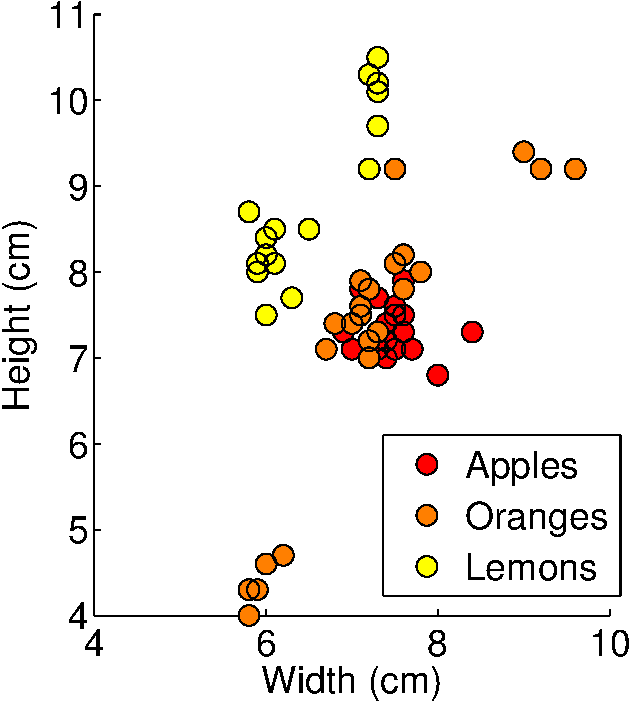
\includegraphics[width=0.5\textwidth]{fruit}
\caption{Heights and widths of apples, oranges, and lemons.  These fruit were
purchased and measured by Iain Murray:
\url{http://homepages.inf.ed.ac.uk/imurray2/teaching/oranges_and_lemons/}.}
\label{fig:fruit}
\end{figure}
\begin{problem}[Classifying Fruit, 15pts]
Please implement the following:
\begin{itemize}
\item Implement the three-class generalization of logistic regression, also
  known as softmax regression, for these data. You will do this by implementing
  gradient descent on the log likelihood. 
\item After this, implement a simple generative classifier with Gaussian
  class-conditional densities, as in Bishop Section 4.2.2. In particular, make
  two implementations of this, one with a shared covariance matrix across all of
  the classes, and one with a separate covariance being learned for each class.
  Note that the staff implementation can switch between these two by the
  addition of just a few lines of code. The shared covariance matrix case is
  detailed in Bishop (and you worked on it in Problem 2), and the separate covariance 
  case is only slightly different. In the separate covariance matrix case, the MLE for the
  covariance matrix of each class is simply the covariance of the data points assigned to that
  class, without combining them as in the shared case.
\end{itemize}
You may use anything in  numpy or scipy, except for scipy.optimize. That being said, if you happen to find a function in numpy or scipy that seems like it is doing too much for you, run it by a staff member. In general, linear algebra and random variable functions are fine. The controller file is problem3.py, in which you will specify parameters. The actual implementations you will write will be in LogisticRegression.py and GaussianGenerativeModel.py.


You will be given unimplemented class interfaces for GaussianGenerativeModel and LogisticRegression in the distribution code, 
and the code will indicate certain lines that you should not change in your final submission. Naturally, don't change these.
These classes will allow the final submissions to have consistency. There will also be a few hyperparameters that are set to
irrelevant values at the moment. You may need to modify these to get your methods to work.
The classes you implement follow the same pattern as scikit-learn, so they should be familiar to you. The distribution code currently outputs nonsense predictions just to show what the high-level interface should be, so you should completely remove the given predict() implementations and replace them with your implementations.

\begin{itemize}
\item The visualize() method for each classifier will save a plot that will show the decision boundaries. Please include those in this assignment.
\item Which classifiers model the distributions well? 
\item What explains the differences?
\end{itemize}
\end{problem}

\subsection*{Solution}

The Gaussian Generative Models (GGMs) both seem to model the distribution better than the Logistic Regression plot, based on simple observation of our visualizations. Firstly, in the Logistic Regression plot, there is a binary divisor between classes and one particular class - indicated in red - seems to dominate the classification (i.e. the algorithm allocates all points to the red class) when we use the given $\lambda$ parameter 1. Indeed, reducing this parameter betters our predictions substantially, but in future analyses we ought to choose $\lambda$ using cross-validation. By contrast, the GGMs display some separation between classes outright. For example, the predictions in the individually estimated covariance GGM are mostly in line with their observed counterparts; all green and red values lie within their respective boundaries with some overlap in the blue values. The shared covariance GGM shows similar precision in its predicted values, especially considering the more narrow range for the blue values. Again, there is some seemingly unavoidable overlap between red and blue classes here. \\

The differences lie mostly in our underlying assumptions about the data. In the GGMs, we assumed the likelihoods could be modeled normally, which we then used to model our posteriors, which informed our predictions. The logistic regression approach did not make such assumptions. Then, we modeled the covariance differently between GGMs. Depending on the question we are trying to answer, shared or individually estimated covariances matrices may be more or less appropriate. For example, if we believe one class will demonstrate substantial variance compared to the others, we ought to account for that in our model with separately estimated covariance matrices. Another possible cause for difference was our use of $\lambda$ in the logistic regression model. Since $\lambda$ was chosen arbitrarily, we could be overfitting. Again, cross-validation is needed to verify this result.  

\begin{figure}[h]
	\centering
	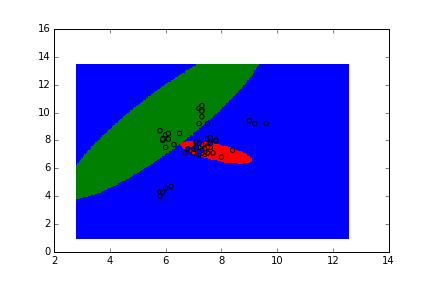
\includegraphics[width=0.5\textwidth]{generative_result_separate_covariances}
	\caption{Generative Gaussian Separate Covariances}.
	\label{fig:separate}
\end{figure}

\begin{figure}[h]
	\centering
	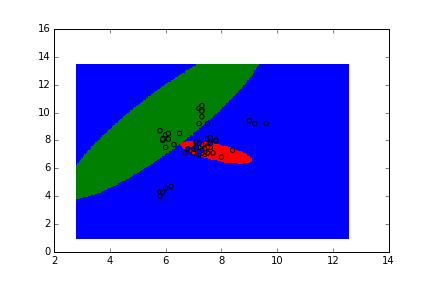
\includegraphics[width=0.5\textwidth]{generative_result_separate_covariances}
	\caption{Generative Gaussian Shared Covariances}.
	\label{fig:shared}
\end{figure}

\begin{figure}[h]
	\centering
	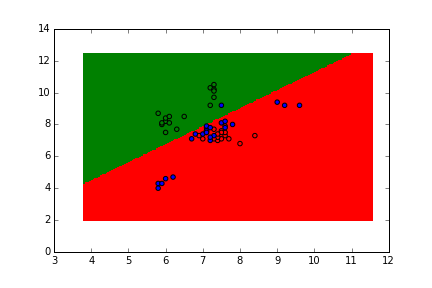
\includegraphics[width=0.5\textwidth]{logistic_regression_result}
	\caption{Logistic Regression}.
	\label{fig:logistic}
\end{figure}

\clearpage
\subsection*{Calibration [1pt]}
Approximately how long did this homework take you to complete? \\
25 hours +


\end{document}
